\documentclass[11pt,a4paper]{article}

% Layout & typography
\usepackage[margin=2.5cm]{geometry}
\usepackage[utf8]{inputenc}
\usepackage[T1]{fontenc}
\usepackage{lmodern}
\usepackage{microtype}
\usepackage{setspace}
\onehalfspacing
\usepackage{titlesec}
\titleformat{\section}{\large\bfseries}{\thesection}{1em}{}
\titleformat{\subsection}{\normalsize\bfseries}{\thesubsection}{1em}{}
\titleformat{\subsubsection}{\normalsize\itshape}{\thesubsubsection}{1em}{}

% Math, symbols, hyperlinks
\usepackage{amsmath,amssymb}
\usepackage[hidelinks]{hyperref}
\usepackage{xurl}
\usepackage{booktabs}
\usepackage{array}
\usepackage{caption}
\captionsetup{font=small,labelfont=bf,labelsep=period,justification=justified}

% Figures
\usepackage{graphicx}
\graphicspath{{../../figures/report/}}
\usepackage{float}

% Code listings (for the small toolbox API snippets)
\usepackage{listings}
\usepackage{xcolor}
\definecolor{codebg}{RGB}{248,248,250}
\definecolor{codekw}{RGB}{59,125,216}
\definecolor{codestr}{RGB}{160,75,75}
\definecolor{codecmt}{RGB}{120,128,140}
\lstdefinestyle{pythonstyle}{
  language=Python,
  basicstyle=\ttfamily\footnotesize,
  keywordstyle=\color{codekw}\bfseries,
  stringstyle=\color{codestr},
  commentstyle=\color{codecmt}\itshape,
  backgroundcolor=\color{codebg},
  frame=single,
  framerule=0pt,
  rulecolor=\color{codebg},
  framesep=4pt,
  xleftmargin=4pt,
  xrightmargin=4pt,
  aboveskip=6pt,
  belowskip=6pt,
  showstringspaces=false,
  breaklines=true,
}
\lstset{style=pythonstyle}

% Citations
\usepackage[numbers,square,sort&compress]{natbib}

\title{\textbf{Coupling methods for multimodal human--nature attunement}\\[0.3em]
\large A toolbox reference}
\author{Antoine Bellemare-Pepin \and Mar Estarellas \and Karim Jerbi \and Michael Lifshitz}
\date{\today}

\begin{document}
\maketitle

\begin{abstract}
\noindent Quantifying how peripheral physiology and cortical activity couple
to the temporal structure of a natural environment is a multimodal,
many-method problem. Differentiating between the existing and rapidly
growing catalogue of coupling methods is itself a challenge: which
method is appropriate depends strongly on the signal properties under
consideration, the hypothesis being tested, and the candidate
physiological mechanism. We propose a two-axis framework that
organises every coupling analysis by (i) the \emph{feature} extracted
from each signal --- raw waveform, oscillatory, or complexity --- and
(ii) the \emph{coupling method} comparing them --- linear, oscillatory,
or information-theoretic. The framework exposes redundancies across
methods (\textit{e.g.}\ ``complexity matching'' turns out to be linear
coupling on a complexity-feature trace) and clarifies when a method is
applicable, when it is misused, and when it overlaps with another. We
instantiate the framework as the Python toolbox \texttt{HNA}
(Human--Nature Attunement), with a modality-agnostic feature subpackage
and a coupling subpackage organised by family. The present document is
a reference: it describes each feature family, each coupling family,
the surrogate-test and group-statistics infrastructure, and a worked
example on real pilot data. Methods presented here are general; they
were developed for the \emph{Multisensory Synchronization as Mechanism
of Nature Connectedness} project but are reusable for any study that
asks how two or more 1-D physiological / sensory signals co-vary in
time.
\end{abstract}

\tableofcontents

\section{Introduction: two axes, not a flat list}

A multimodal coupling analysis always involves two implicit choices:

\begin{enumerate}
  \item \textbf{What aspect of each signal to compare} --- the raw
        waveform, an \emph{oscillatory feature} (envelope, instantaneous
        phase, band-power, FOOOF spectral peaks), or a
        \emph{complexity feature} (DFA scaling exponent, fractal
        dimension, FOOOF aperiodic exponent, multiscale entropy).
  \item \textbf{How to compare them} --- with a \emph{linear},
        \emph{oscillatory}, or \emph{information-theoretic} estimator.
\end{enumerate}

These two choices are independent. Some methods bake the feature step
in (e.g.\ phase-locking value always extracts Hilbert phase first;
phase-amplitude coupling always extracts a slow phase and a fast
amplitude). Others (cross-correlation, mutual information) accept any
1-D input. The framework presented in this report makes the choice
\emph{explicit}: pick a feature per signal, pick a coupling method,
combine. Many named methods then reveal themselves as cells of a
\(3 \times 3\) grid (Figure~\ref{fig:framework}).

A perhaps surprising consequence is that ``complexity'' is naturally a
\emph{feature axis}, not a coupling axis. Every method in the toolbox's
\texttt{coupling.complexity} subpackage --- \texttt{exponent\_matching},
\texttt{fluctuation\_matching}, \texttt{mse\_matching},
\texttt{complexity\_coupling} --- is a \emph{linear} comparison applied
to a complexity feature: a scalar (DFA $\alpha$), a curve indexed by
scale ($F(s)$, MSE($\tau$)), or a trace indexed by time ($\alpha(t)$).
The complexity character lives in the feature; the comparison step is
plain Pearson. Genuine cross-complexity \emph{coupling} estimators
(detrended cross-correlation analysis, multiscale cross-entropy,
multiscale cross-mutual-information) exist in the literature but are
not yet implemented in HNA --- see \S\ref{sec:future} for future work.

The framework also clarifies that ``phase-amplitude coupling'' (PAC) is
\emph{oscillatory} coupling between two \emph{oscillatory} features (a
slow phase and a fast amplitude), and that PLV / wPLI / coherence are
``oscillatory $\times$ oscillatory'' methods even when called on raw
signals --- they implicitly do the Hilbert / Welch step first. The
framework therefore unifies what might otherwise look like an unrelated
catalogue of names.

The HNA toolbox~(\S\ref{sec:toolbox-arch}) ships with at least one
canonical estimator per cell that has a recognised name in the
literature, plus the generic infrastructure --- surrogate testing,
multiple-comparisons correction, cluster permutation, paper-style
plotting --- needed to turn any per-pair coupling number into a
defensible group-level claim.

\begin{figure}[H]
  \centering
  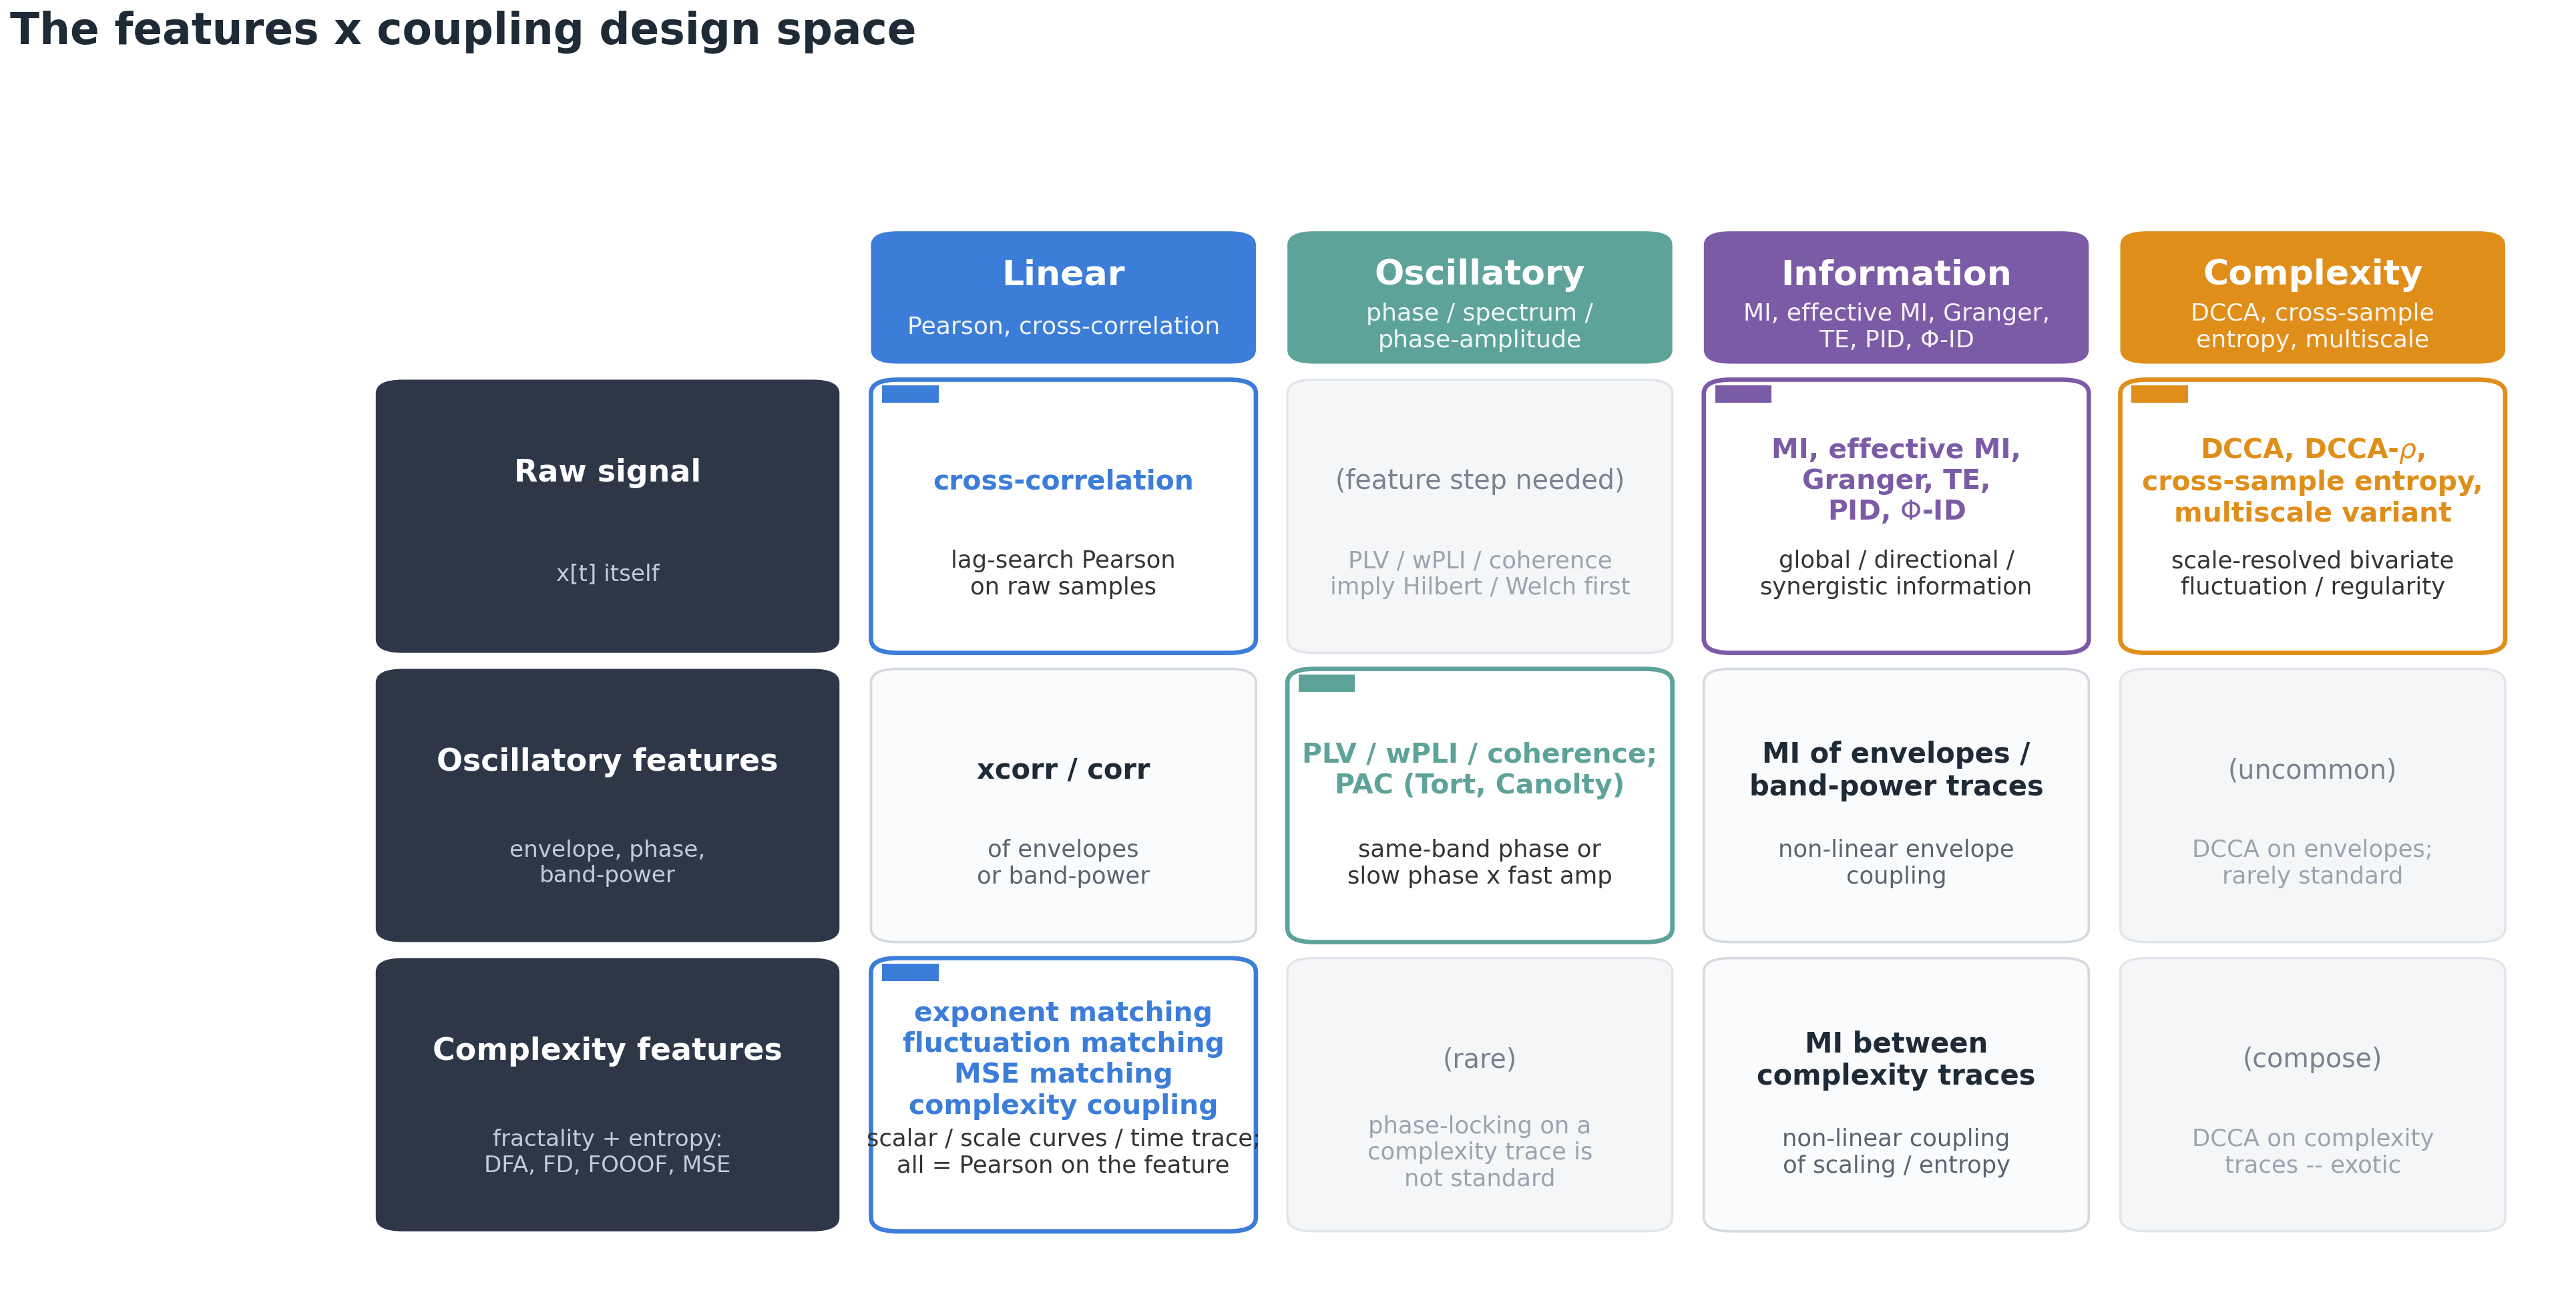
\includegraphics[width=\textwidth]{Methods5_features_x_coupling.png}
  \caption{\label{fig:framework}\textbf{The features $\times$ coupling
    design space.} Three feature families (rows) crossed with three
    coupling-method families (columns). Cells outlined and labelled in
    colour are named, ready-to-use methods in the HNA toolbox; lighter
    cells describe the general pattern; faded cells flag uncommon or
    not-standard combinations. The ``raw signal $\times$ oscillatory''
    cell is intentionally faded --- in practice the named methods that
    look like ``oscillatory on the raw signal'' (PLV, wPLI, coherence)
    embed a Hilbert / Welch feature step and therefore actually live in
    the ``oscillatory features $\times$ oscillatory'' cell one row
    down. The bottom-left cell carries all four toolbox-named
    complexity methods --- exponent matching, fluctuation matching,
    MSE matching, and complexity coupling --- because they are all
    linear comparisons applied to a complexity feature, varying only
    in which observable of complexity (scalar, scale-resolved curve,
    or time-resolved trace) is compared.}
\end{figure}

\section{Notation and toolbox layout}

We write $x[t]$, $y[t]$ for two 1-D signals sampled at rate $f_s$. A
\emph{feature transformation} produces a derived signal $\phi(x)[t]$ that
is itself 1-D (envelope, phase, band-power, scaling exponent\ldots) or
sometimes multi-dimensional (one channel of $\alpha(t)$ per EEG channel;
a vector of band powers per window). A \emph{coupling estimator} consumes
two such features and returns a scalar (or a time series of scalars):
\(\kappa\bigl(\phi_X(x),\phi_Y(y)\bigr)\). When $\phi$ is the identity
(no feature step), the estimator operates on the raw signals.

The HNA toolbox lays out this structure directly:
\begin{itemize}
  \item \texttt{HNA.dsp} --- generic primitives (filters, NaN
        interpolation, Hilbert envelope, $z$-score, resample).
  \item \texttt{HNA.modalities} --- per-signal cleaners (audio
        envelope decomposition, EEG bandpass + channel iteration,
        respiration cleaning, ECG cleaning + R-peak detection +
        windowed HRV).
  \item \texttt{HNA.features} --- modality-agnostic feature extractors:
        Welch PSD bands, entropy, fractal exponents, FOOOF aperiodic,
        and a generic \texttt{windowed\_channel\_features} iterator.
  \item \texttt{HNA.coupling} --- coupling estimators, organised into
        four submodules (\texttt{linear}, \texttt{oscillatory},
        \texttt{information}, \texttt{complexity}). The first three
        match the three coupling-method columns of
        Figure~\ref{fig:framework}; the fourth (\texttt{complexity})
        is an organisational unit for the four methods that operate
        \emph{on} complexity features --- conceptually they are linear
        comparisons (cf.\ \S4.4). The package \texttt{\_\_init\_\_}
        re-exports the full public API so any method is reachable as
        \texttt{from HNA.coupling import \ldots}.
  \item \texttt{HNA.surrogates} --- phase-shuffle and time-shift
        generators plus a generic surrogate-test harness.
  \item \texttt{HNA.stats} --- linear, repeated-measures, circular,
        and cluster-based permutation statistics.
  \item \texttt{HNA.viz} --- paper-ready style + canonical condition
        palette + reusable plot helpers (forest, polar, spectrum,
        topomap).
\end{itemize}

\section{Feature families}

\subsection{Raw signal}

The samples themselves, after cleaning. ``Raw'' here means
\emph{post-preprocessing}: the audio waveform after envelope
extraction~\cite{NK2}, the respiration trace after a 0.05--1\,Hz
band-pass and $z$-score, the ECG after NeuroKit2 cleaning and R-peak
detection~\cite{NK2,Pichot}. Coupling on raw signals is appropriate when
you want to test direct sample-by-sample dependence (linear
correlation, mutual information, Granger). It is \emph{not} appropriate
for asking ``do these signals share a 0.20\,Hz oscillation?''; that
question lives in oscillatory features.

\subsection{Oscillatory features}

Anything that exposes the frequency or phase content of a signal. The
toolbox provides:

\begin{itemize}
  \item \textbf{Hilbert envelope and instantaneous phase} ---
        \texttt{dsp.hilbert\_envelope}, plus the Hilbert step embedded
        inside \texttt{coupling.oscillatory.\_phase\_and\_amp}.
  \item \textbf{Audio band-organised envelopes} ---
        \texttt{modalities.audio.decompose\_envelope} returns a 12-band
        envelope set (broad / swell-0.1\,Hz / swell-0.2\,Hz / HRV-LF /
        HRV-HF / splash / EEG~$\delta$/$\theta$/$\alpha$/$\beta$/$\gamma_1$),
        all on a 256\,Hz time axis.
  \item \textbf{Welch PSD band-power} ---
        \texttt{features.psd.welch\_band\_powers} integrates a Welch
        PSD over user-specified bands, returning one scalar per band
        per window. The default \texttt{EEG\_BANDS} are 2--4, 4--8,
        8--13, 13--20, 20--30, and 30--50\,Hz.
  \item \textbf{FOOOF spectral peaks} ---
        \texttt{features.aperiodic.fit\_aperiodic\_psd} returns the
        list of detected peaks (centre frequency, power, bandwidth)
        in addition to the aperiodic offset/exponent.
\end{itemize}

\begin{lstlisting}
from HNA.modalities.audio import decompose_envelope
from HNA.features.psd import welch_band_powers, EEG_BANDS

# 12-band audio envelope (256 Hz, time-aligned to physio)
df, fs = decompose_envelope(wav_path)

# Welch band powers on a 5-s EEG window
bp = welch_band_powers(eeg_window, fs=256, bands=EEG_BANDS)
# -> {"delta_abs": ..., "alpha_rel": ..., ...}
\end{lstlisting}

\subsection{Complexity features}

Two related but distinct sub-types, both of which the toolbox treats as
``complexity'':

\begin{itemize}
  \item \textbf{Fractality / scaling exponents} ---
        \texttt{features.fractal} provides Higuchi, Katz, Petrosian
        fractal dimensions, the DFA scaling exponent
        $\alpha$~\cite{Peng}, and a Hurst exponent via
        rescaled-range. \texttt{features.aperiodic} adds the
        FOOOF~\cite{Donoghue2020} aperiodic exponent (the slope of the
        log-log PSD after peak removal). All return one scalar per
        window; sliding the window over time gives a scaling-exponent
        \emph{trace} that captures non-stationary changes in
        long-range structure.
  \item \textbf{Entropy / regularity} ---
        \texttt{features.entropy} provides Lempel--Ziv complexity,
        permutation entropy, spectral entropy, SVD entropy and sample
        entropy. The toolbox also includes a multiscale
        sample-entropy curve in
        \texttt{coupling.complexity.mse\_curve}~\cite{Costa2002}.
\end{itemize}

The unifying property is that complexity features describe \emph{how}
the signal fluctuates across scales (fractality) or how regular it is
(entropy), rather than its instantaneous amplitude or phase. They are
the natural axis for ``complexity matching'' analyses.

\begin{lstlisting}
from HNA.features.fractal import dfa_alpha, hurst_rs, all_fractals
from HNA.features.entropy import all_entropies
from HNA.features.aperiodic import aperiodic_features

dfa_alpha(x)                  # scalar
hurst_rs(x)                   # scalar
all_fractals(x)               # dict: higuchi_fd, dfa_alpha, ...
all_entropies(x, fs=256)      # dict: lzc, perm_entropy, ...
aperiodic_features(x, fs=256) # FOOOF on Welch PSD
\end{lstlisting}

\section{Coupling families}
\label{sec:coupling}

This section defines each family and lists the canonical estimators. We
keep the math light: one defining expression per method plus an
intuition. Figure~\ref{fig:onepair} runs every family on the same
synthetic signal pair.

\begin{figure}[H]
  \centering
  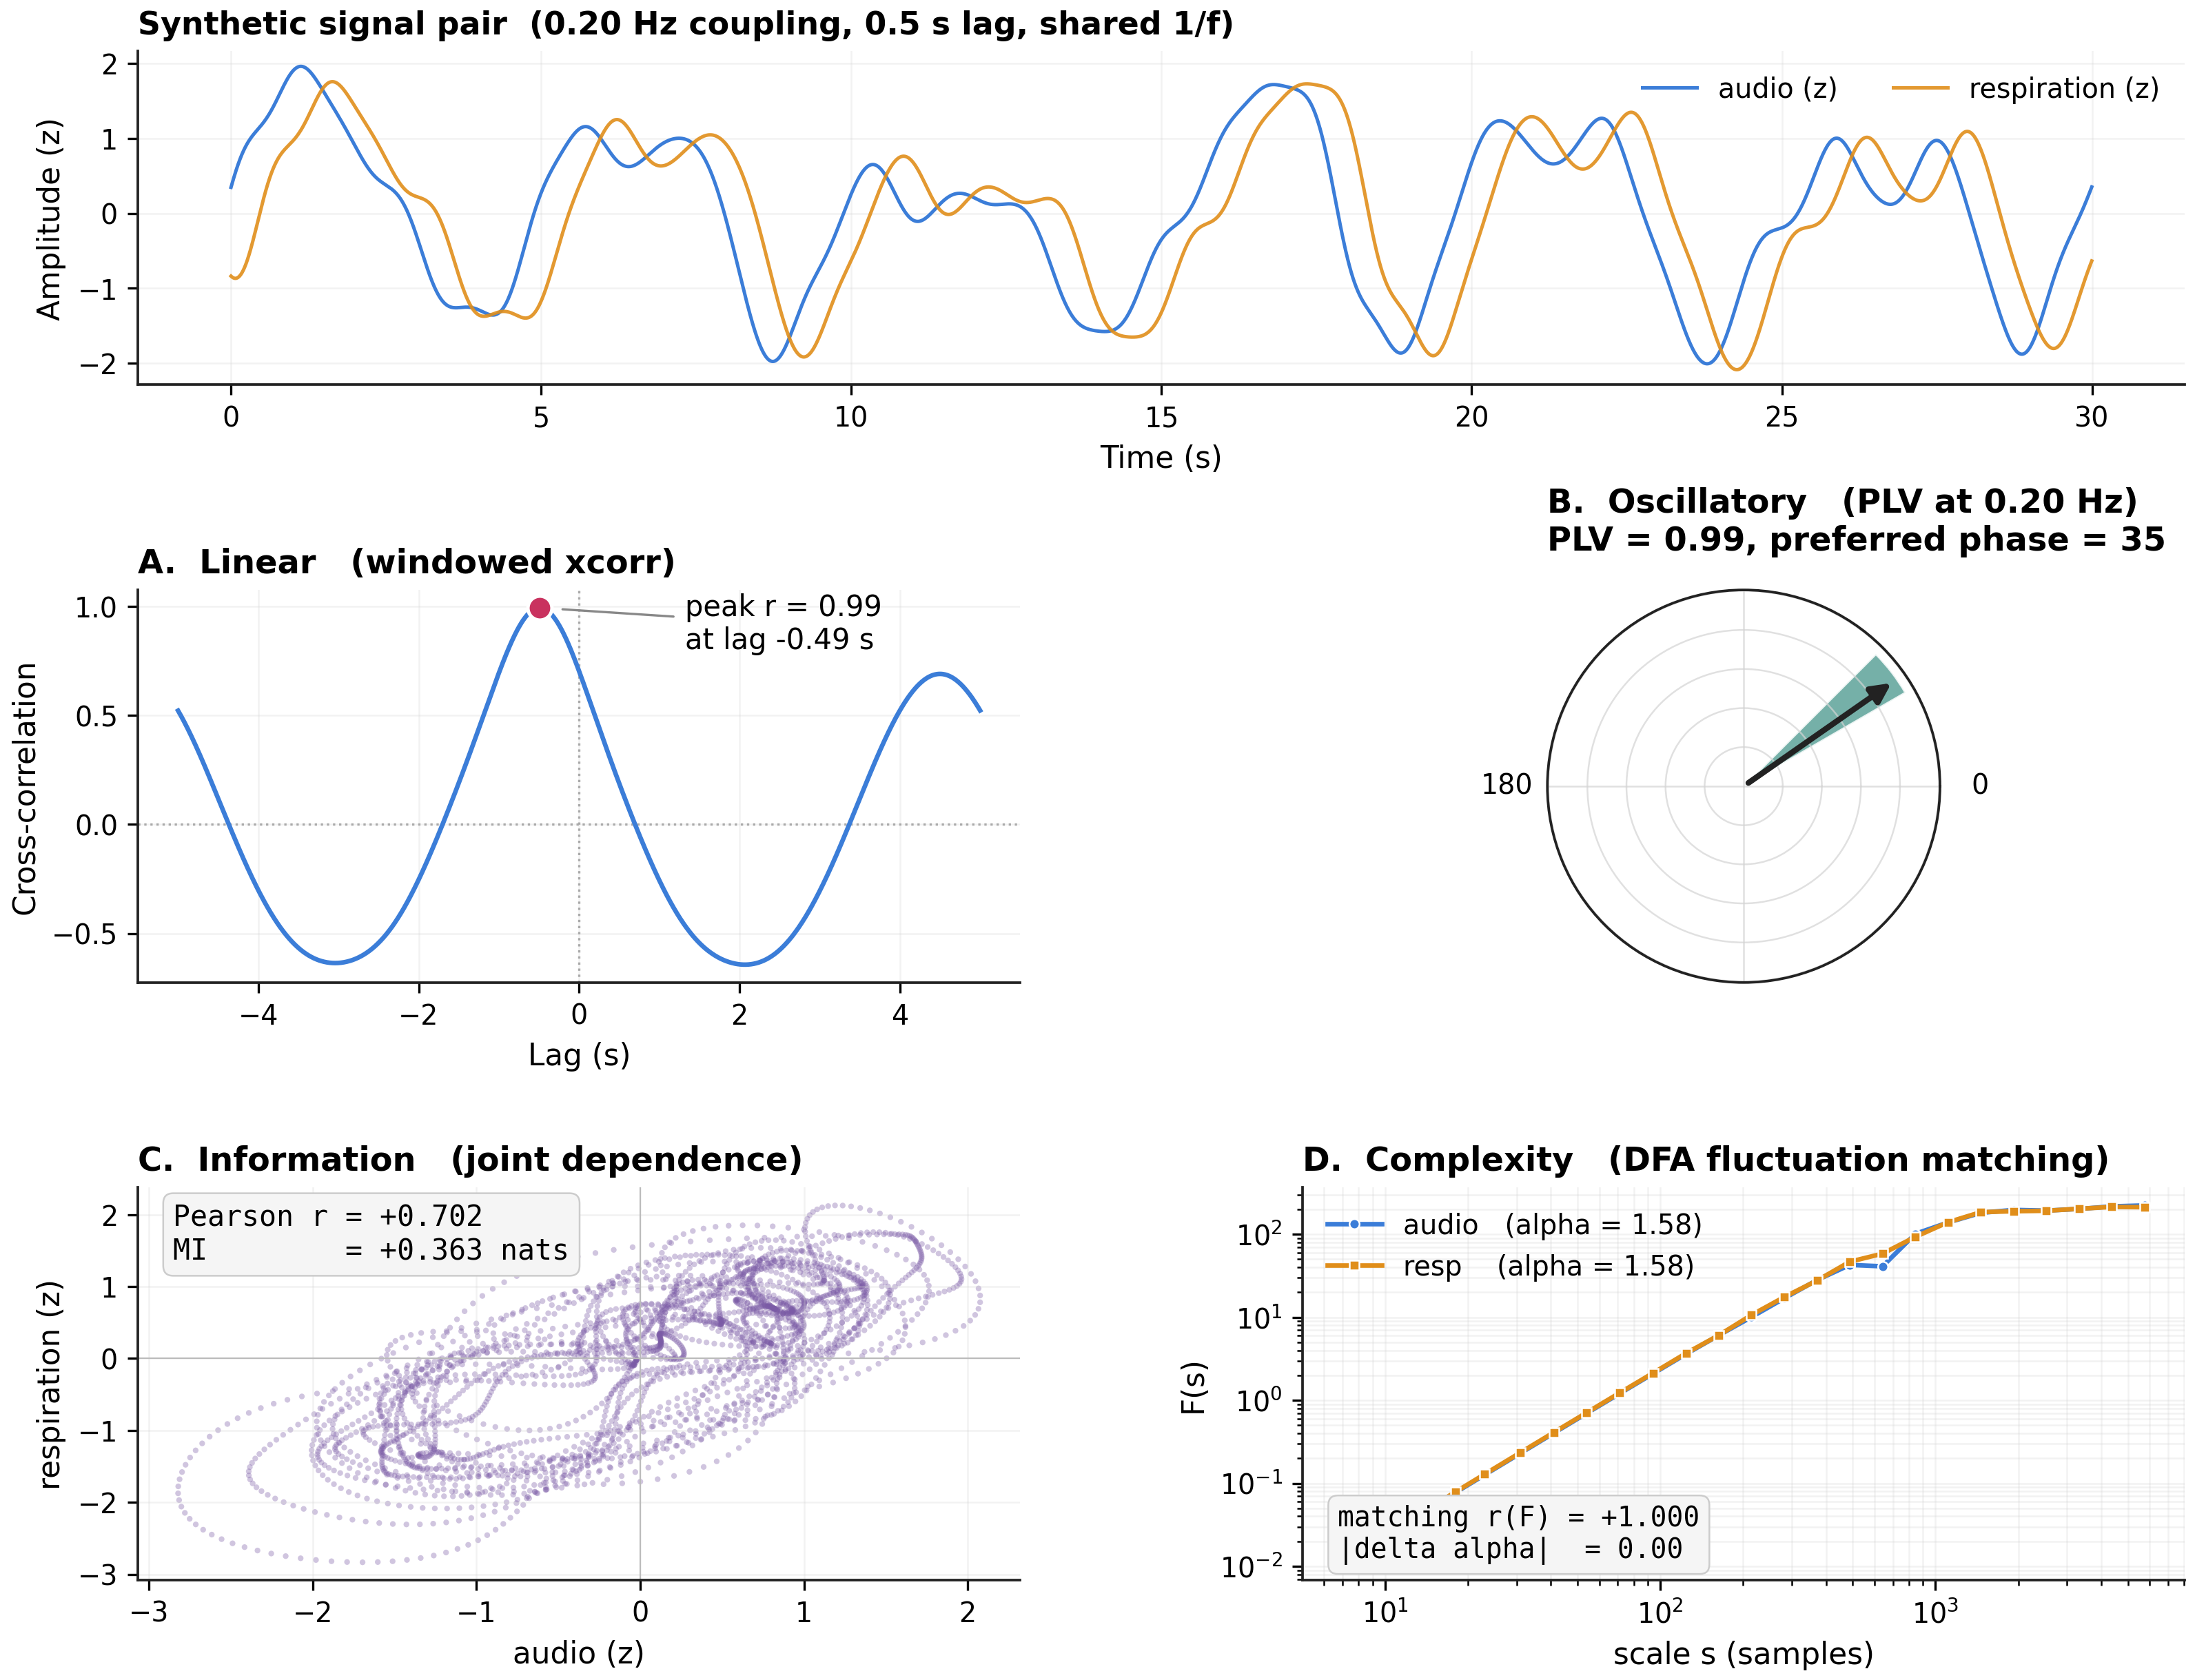
\includegraphics[width=\textwidth]{Methods1_coupling_families.png}
  \caption{\label{fig:onepair}\textbf{Each coupling family on the same
    synthetic pair.} A constructed audio-vs-respiration pair (top)
    coupled at 0.20\,Hz with a 0.5\,s phase lag, viewed through one
    canonical estimator per family. \textbf{A. Linear} ---
    cross-correlation peaks at $r=0.99$ at $\text{lag}=-0.5$\,s.
    \textbf{B. Oscillatory} --- PLV at 0.20\,Hz is 0.99 with
    preferred-phase $35^\circ$ (matching the constructed lag).
    \textbf{C. Information} --- joint scatter shows clear dependence;
    Pearson and MI both positive. \textbf{D. Complexity} --- both
    signals share scaling exponent $\alpha = 1.58$, fluctuation curves
    overlap.}
\end{figure}

\subsection{Linear family --- windowed cross-correlation}

The simplest family: time-domain linear amplitude alignment, possibly
with a time lag. The toolbox ships
\texttt{coupling.linear.windowed\_xcorr}, which slides a window over
the two signals and reports the per-window peak Pearson correlation
within $\pm \tau_{\max}$ lag and the lag at which it occurs:
\begin{equation}
\label{eq:xcorr}
r_{\max}(t) \;=\; \max_{|\tau|\le\tau_{\max}}\;
\frac{1}{W}\sum_{s=0}^{W-1} \tilde{x}[t + s]\,\tilde{y}[t + s + \tau],
\qquad \tilde{x}\equiv\tfrac{x-\bar x}{\sigma_x}.
\end{equation}
Use the lag-search variant when the two signals are physically separated
(sound takes time to act on the body); use a lag-zero Pearson when you
want to isolate \emph{linear amplitude} from \emph{phase} coupling
(e.g.\ a $90^\circ$ phase-locked pair has $r_{\max}\approx 1$ but
$r_{\text{lag-zero}}\approx 0$; cf.\ Methods Fig.~3, case 2).

\begin{lstlisting}
from HNA.coupling import windowed_xcorr
xc = windowed_xcorr(x, y, fs=256, win_sec=120, step_sec=10, max_lag_sec=10)
# xc.peak_r, xc.peak_lag_s, xc.times_s
\end{lstlisting}

\subsection{Oscillatory family --- coherence, PLV, wPLI, PAC}

Coupling in the frequency or phase domain.

\paragraph{Welch coherence.}
\(C_{xy}(f) = |S_{xy}(f)|^2 / (S_{xx}(f)\,S_{yy}(f))\), the
magnitude-squared coherence. \texttt{coupling.oscillatory.band\_coherence}
returns the spectrum, the band-averaged coherence, the peak frequency
within band, and (optionally) a windowed band-averaged time series.

\paragraph{Phase-locking value (PLV)}~\cite{Lachaux1999}.
For two band-pass-filtered signals at the same target frequency $f_0$,
let $\Delta\varphi[t]$ be the wrapped instantaneous phase difference of
the two analytic signals. Then
\begin{equation}
\text{PLV} \;=\; \biggl|\, \frac{1}{N}\sum_{t=1}^{N}\, e^{i\,\Delta\varphi[t]} \,\biggr|.
\end{equation}
PLV is in $[0,1]$; $1$ is perfect phase locking. The toolbox auto-detects
$f_0$ from the dominant Welch peak of the second signal if not given.

\paragraph{Weighted phase-lag index (wPLI)}~\cite{Vinck2011}.
A debiased relative of PLV that is insensitive to common-source zero-lag
contamination. With $S = \mathrm{Im}\bigl(e^{i\Delta\varphi}\bigr)$:
\begin{equation}
\text{wPLI} \;=\; \frac{|\langle S\rangle|}{\langle |S|\rangle}.
\end{equation}

\paragraph{Phase-amplitude coupling (PAC)}~\cite{Tort2010,Canolty2006}.
Test whether the slow-band phase of one signal organises the fast-band
amplitude of the other. With $\phi_{\text{lo}}[t]$ the Hilbert phase of
$x$ in the low band and $A_{\text{hi}}[t]$ the Hilbert amplitude of $y$
in the high band, the toolbox provides two estimators:
\begin{itemize}
  \item \textbf{Tort modulation index}: bin $A_{\text{hi}}$ by phase
        $\phi_{\text{lo}}$ into $N$ bins, normalise the per-bin mean
        amplitude into a probability distribution $P$, and report
        $\mathrm{MI} = (\log N - H(P))/\log N \in [0,1]$. Tort MI
        captures the \emph{shape} of the phase-binned amplitude
        distribution and is amplitude-blind: tiny filter residuals can
        give large MI if their distribution happens to be uneven.
  \item \textbf{Canolty mean vector length}:
        $\bigl|\langle A_{\text{hi}}\, e^{i\phi_{\text{lo}}}\rangle\bigr|$,
        optionally normalised by $\langle A_{\text{hi}}\rangle$. The raw
        MVL is amplitude-aware and therefore much more robust to
        filter-residual leakage; we use it as the default PAC estimator.
\end{itemize}

\begin{lstlisting}
from HNA.coupling import (
    band_coherence_windowed, plv_phase_sync, windowed_plv,
    wpli_phase_sync, windowed_wpli, canolty_mvl, comodulogram,
)

plv = plv_phase_sync(env, resp, fs=256, bw_hz=0.10).plv
mvl = canolty_mvl(eeg_low, eeg_high, fs=256,
                  low_band=(4, 8), high_band=(30, 50)).mvl
\end{lstlisting}

\subsection{Information family --- MI, effective MI, Granger, transfer entropy}

Probabilistic and directional dependence.

\paragraph{Mutual information (MI).}
$I(X;Y) = \int p(x,y) \log\!\bigl(p(x,y) / (p(x)p(y))\bigr)\,dx\,dy$,
estimated with the kNN/Kraskov-style estimator from
\texttt{sklearn.feature\_selection.mutual\_info\_regression}~\cite{Kraskov2004}.
A practical caveat: the kNN MI estimator is biased upward on
auto-correlated time series, because it assumes i.i.d.\ samples. The
toolbox's \texttt{coupling.information.windowed\_mi} reports the raw
estimate; for absolute values we recommend (a)~decorrelating
downsampling before the call (e.g.\ keep every $f_s/4$-th sample), or
(b)~the bias-corrected variant below.

\paragraph{Effective mutual information.}
\(I_{\text{eff}} = I(X;Y) - \overline{I(X; \tilde Y)}\), where $\tilde Y$
is a phase-shuffled surrogate of $Y$ that preserves $Y$'s spectrum but
breaks the temporal relationship to $X$. The bias from shared spectral
structure cancels.

\paragraph{Granger causality.}
A linear-Gaussian special case of transfer entropy. The toolbox fits a
bivariate VAR via \texttt{statsmodels} and reports F-statistics for
``$X$~Granger-causes~$Y$'' and the reverse, plus a signed score
\(\log_{10}p_{Y\to X} - \log_{10}p_{X\to Y}\) (positive $\Rightarrow$
$X$ drives $Y$). Granger is \emph{linear}; for non-Gaussian or non-linear
direction, the toolbox includes a stub for kNN-based transfer
entropy~\cite{Schreiber2000} that loads the optional \texttt{copent}
dependency lazily.

\begin{lstlisting}
from HNA.coupling import (
    windowed_mi, effective_mi, granger_bivariate, granger_score,
)

raw_mi  = windowed_mi(x, y, fs=256, win_sec=60)
em      = effective_mi(x, y, fs=256, n_surrogates=200)
gb      = granger_bivariate(x, y, max_lag=10, ic="aic")
\end{lstlisting}

\subsection{Linear coupling on complexity features}

Despite the toolbox subpackage being called \texttt{coupling.complexity},
\emph{every method here is a linear comparison applied to a complexity
feature}. The complexity character lives in the feature; the comparison
step itself is a Pearson correlation (or, in the scalar case, a
$|\Delta|$ similarity). What distinguishes the four toolbox methods is
which \textbf{observable of complexity} they compare:

\begin{center}
\renewcommand{\arraystretch}{1.25}
\begin{tabular}{>{\bfseries}lll}
\toprule
Observable & What it is & Toolbox method \\
\midrule
Scalar      & one number per signal ($\alpha$, FD, Hurst)
            & \texttt{exponent\_matching} \\
Curve over scales & vector indexed by scale $s$ or coarse-grain $\tau$
            & \texttt{fluctuation\_matching}, \texttt{mse\_matching} \\
Trace over time   & vector indexed by window centre
            & \texttt{complexity\_coupling} \\
\bottomrule
\end{tabular}
\end{center}

\paragraph{Static scalar match --- \texttt{exponent\_matching}.}
Compute one scalar complexity measure per signal (typically DFA
$\alpha$, Hurst, or FOOOF aperiodic exponent) and report:
\(\mathrm{matching} = 1 - |\alpha_x - \alpha_y|/\alpha_{\max} \in [0,1]\),
with $\alpha_{\max}=2$ by default. The most direct test of ``do the two
signals share scaling structure?''. There is no trace and no curve ---
just two numbers compared.

\paragraph{Static curve match --- \texttt{fluctuation\_matching},
\texttt{mse\_matching}.}
DFA fluctuation function $F(s)$ versus scale $s$, or multiscale
sample-entropy MSE($\tau$) versus coarse-graining factor $\tau$,
computed for each signal; the two curves are then compared via the
Pearson correlation across scales (in log--log for $F(s)$). This is
``linear coupling at the \emph{scale} axis'': it asks whether the two
signals' complexity profile has the same shape across scales. More
diagnostic than the scalar match because it picks up matching at some
scales but not others.

\paragraph{Dynamic trace coupling --- \texttt{complexity\_coupling}.}
Slide a window over each signal, compute a scalar complexity per window
(default DFA $\alpha$), and Pearson-correlate the resulting traces:
\begin{equation}
r_{\text{complex}}\;=\;\mathrm{Pearson}\!\bigl(\alpha_X(t),\,\alpha_Y(t)\bigr).
\end{equation}
\textbf{This is ``linear coupling at the \emph{time} axis'' --- the
identity that makes the framework click}: the toolbox function
\texttt{complexity\_coupling} is literally
\texttt{windowed\_exponent}~$\to$~Pearson, which is linear coupling on
a complexity-feature trace. Stationary signal pairs give
$r_{\text{complex}}\approx 0$; signals whose scaling \emph{drifts
together over time} give large $r_{\text{complex}}$, even when their
amplitudes and phases are unrelated~(\cite{Marmelat2012}; cf.\ Methods
Fig.~3 case~5). Of the four methods in this section it is the only one
that is genuinely time-resolved, and the only one that can in principle
take a non-linear coupling metric in place of Pearson (e.g.\ MI on the
two $\alpha(t)$ traces) --- this is exposed via the \texttt{method=}
keyword.

\begin{lstlisting}
from HNA.coupling import (
    exponent_matching, fluctuation_matching, mse_matching,
    windowed_exponent, complexity_coupling,
)

m  = exponent_matching(x, y)             # scalar similarity
fm = fluctuation_matching(x, y)          # F(s) curve correlation
me = mse_matching(x, y)                  # MSE(tau) curve correlation
cc = complexity_coupling(x, y, fs=256,   # alpha(t) trace coupling
                          win_sec=30, step_sec=5)
\end{lstlisting}

\paragraph{What this section is \emph{not}.}
None of the methods above is a genuine cross-complexity coupling
estimator in the sense of detrended cross-correlation analysis (DCCA),
multiscale cross-entropy, or multiscale cross-mutual-information. Those
would have a non-linear, scale-aware \emph{coupling step} (not just a
non-linear feature). They are noted in \S\ref{sec:future} as the
natural next addition to the toolbox.

\section{Surrogate testing}

A coupling number on its own is uninterpretable: $\mathrm{PLV}=0.4$ may
be remarkable for one signal pair and unremarkable for another. The
toolbox provides surrogate-data hypothesis testing through
\texttt{HNA.surrogates}.

\paragraph{Phase-shuffle surrogate.} Randomises the phase of every
non-DC, non-Nyquist Fourier bin of one signal, leaving its magnitude
spectrum exactly intact. Use this when you want to control for shared
spectral structure (the most common case).

\paragraph{Time-shift surrogate.} Circularly shifts one signal by a
random offset. Cheaper and assumption-light, but only valid when the
signal is reasonably stationary across the window.

\paragraph{Generic harness.}
\texttt{surrogate\_test(metric\_fn, x, y, n=500, method="phase\_shuffle")}
returns the observed metric, the full null distribution, an
add-one--corrected one-sided $p$-value, and a $z$-score relative to the
null. It accepts \emph{any} callable returning a scalar, so it works
out-of-the-box for every method in the previous section --- phase-locking
value, PAC, mutual information, Granger score, complexity coupling.

\paragraph{Choosing the right null.} Phase-shuffle is intentionally
conservative for phase-/complexity-family methods, because it preserves
the very spectrum on which those methods rely. For PLV/wPLI/PAC, a
\emph{time-shift} surrogate is more discriminative; for fluctuation
matching, a \emph{sample-shuffle} (which destroys autocorrelation) is
the only null that meaningfully breaks the matched scaling.

\section{Group statistics}

Per-(subject, condition) coupling values are aggregated into group claims
through \texttt{HNA.stats}:

\begin{itemize}
  \item \textbf{Fisher $z$-transform} (\texttt{fisher\_z}, \texttt{inv\_fisher\_z}) for
        sample-mean Pearson statistics.
  \item \textbf{BH-FDR} (\texttt{fdr\_bh}) for mass-univariate
        multiple-comparisons correction (e.g.\ across EEG channels).
  \item \textbf{Friedman omnibus + paired Wilcoxon post-hoc}
        (\texttt{friedman\_with\_posthoc}) for repeated-measures
        condition contrasts in small-$N$ designs.
  \item \textbf{Circular Rayleigh test} (\texttt{rayleigh\_test}) for
        non-uniformity of preferred phases.
  \item \textbf{Cluster-based permutation testing}
        (\texttt{cluster\_permutation\_paired\_1d} and the two-sample
        twin) for time- or frequency-resolved repeated-measures
        contrasts; Maris/Oostenveld convention~\cite{MarisOostenveld2007}
        with sign-flip permutations.
\end{itemize}

The standard pipeline for a windowed coupling time series is:
\emph{(i)} per-subject windowed metric trace, \emph{(ii)} cluster
permutation against zero (or against a baseline condition), \emph{(iii)}
optional Friedman + post-hoc Wilcoxon on the per-subject means with
BH-FDR across modalities or channels.

\section{Questions and guidelines}
\label{sec:guidelines}

This section is the practical companion to \S\ref{sec:coupling}: which
method makes sense for which question, what signal properties are
required, and where each method tends to mislead.

\subsection{What does each family actually detect?}

Figure~\ref{fig:cases} shows five clearly distinct coupling scenarios
with each canonical estimator's response. The take-home: \emph{no
single method is best}. Pearson alone misses phase coupling at
$90^\circ$; PLV alone misses non-linear and complexity coupling; mutual
information alone misses pure phase locking when amplitudes are
uncorrelated; complexity matching fires on signals whose
\emph{scaling} co-drifts, even when amplitudes never touch.

\begin{figure}[H]
  \centering
  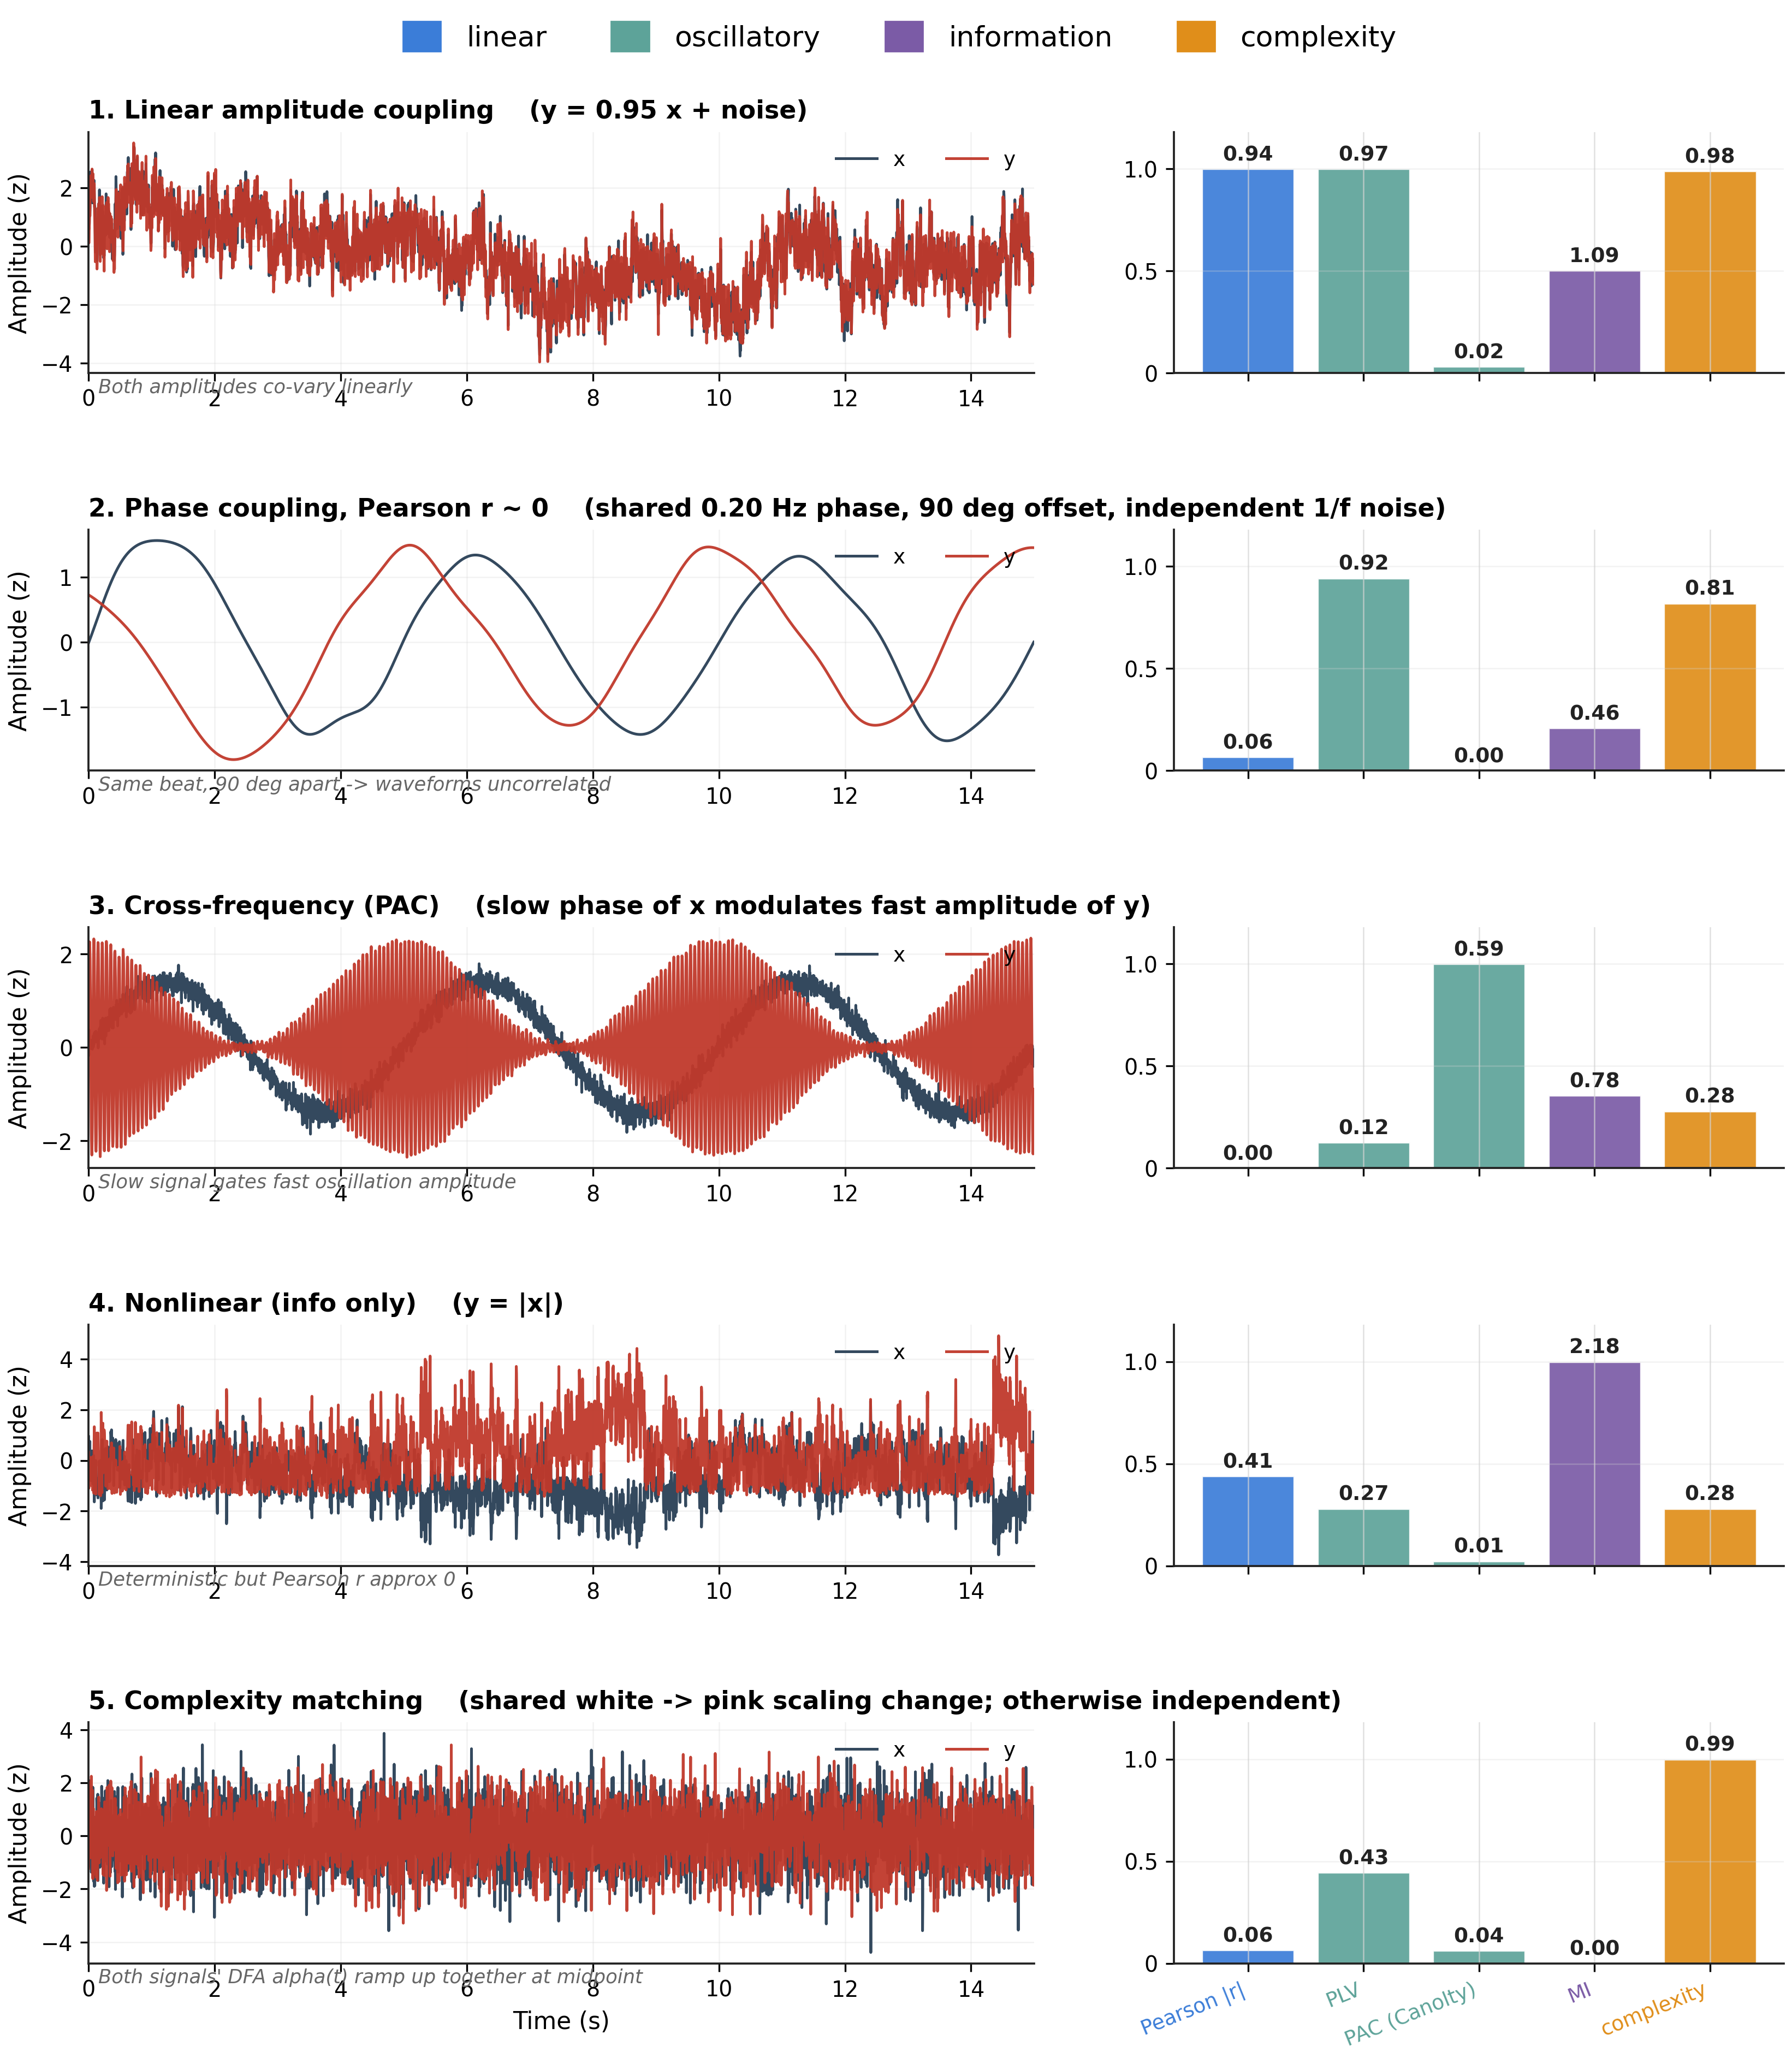
\includegraphics[width=\textwidth]{Methods3_coupling_cases.png}
  \caption{\label{fig:cases}\textbf{Five clear coupling scenarios.}
    Left column: synthetic signal pair (15\,s preview).
    Right column: each method's response, scaled to the method's
    maximum across cases (raw value annotated above each bar). The
    ``coupling family'' colour code matches every figure in this
    report. Each case has a single-method peak corresponding to the
    family it was constructed to exemplify.}
\end{figure}

\subsection{Signal properties that enable / forbid a method}

\begin{itemize}
  \item \textbf{Length and stationarity.} PLV, wPLI and coherence need
        many cycles of the target frequency (a 0.20\,Hz coupling needs
        $\geq 60$\,s for a stable PLV; PAC needs the same on the slow
        side and many fast cycles per slow cycle). Complexity
        estimators degrade on short signals: DFA needs $\geq 1000$
        samples per scale; FOOOF needs broadband content; multiscale
        entropy degrades quickly past $\tau\!=\!10$ on short data.
  \item \textbf{Broadband content.} FOOOF aperiodic and DFA require
        broadband 1/f-ish content. After a steep band-pass, both will
        be ill-defined --- the toolbox flags low fit
        $R^2$ as ``narrow-band'' and refuses to draw an aperiodic
        slope.
  \item \textbf{Dominant frequency.} Coherence/PLV/wPLI need a
        dominant-frequency choice. The toolbox auto-picks the Welch peak
        of the second signal, but you should override
        (\texttt{f0=...}) if the auto-pick is unstable.
  \item \textbf{Auto-correlation.} The kNN MI estimator is biased
        upward on auto-correlated waveforms. Decorrelate by
        downsampling before the MI call, or report effective MI
        instead of raw.
  \item \textbf{Outliers, drift, NaNs.} Cross-correlation and
        coherence are robust if the toolbox's defaults are kept (linear
        detrend, $z$-score, NaN interpolation). Granger requires
        explicit detrending; the toolbox does this for you when
        \texttt{detrend=True} (default).
\end{itemize}

\subsection{Common misuses and design notes}

The HNA defaults make a few opinionated choices. Each is documented as
a one-liner here in case the reader wants to reproduce or override.

\begin{itemize}
  \item \emph{We default to Canolty MVL, not Tort MI, for PAC.}
        Tort MI is amplitude-blind and inflates on filter residuals
        whose tiny amplitude is shape-aligned with the slow phase by
        chance.
  \item \emph{We decorrelate-downsample before kNN MI estimation.}
        sklearn's MI estimator is biased upward on autocorrelated
        time series; downsampling to roughly the autocorrelation
        time-scale yields meaningful absolute values.
  \item \emph{We use lag-zero Pearson, not lag-search xcorr, when
        differentiating linear from phase coupling.} A lag-search
        xcorr finds an alignment lag for any same-frequency pair,
        which can confuse ``linear amplitude coupling'' with ``phase
        coupling'' (Methods Fig.~3, cases 1--2).
  \item \emph{We compose ``complexity coupling'' as
        \texttt{windowed\_exponent} $\to$ Pearson.} This is exactly
        ``linear coupling applied to the complexity-feature trace'',
        and it surfaces shared time-varying scaling structure between
        otherwise independent signals (Methods Fig.~3, case 5).
  \item \emph{We restrict FOOOF aperiodic fits to $\geq 1$\,Hz.}
        The very low frequencies, especially after a sharp low-pass,
        are dominated by filter rolloff and inflate the slope estimate.
  \item \emph{We treat ``raw signal $\times$ oscillatory''
        cells as a feature step.} PLV, wPLI and coherence implicitly
        do Hilbert/Welch and therefore live one row down in the
        framework (cf.\ Figure~\ref{fig:framework}).
\end{itemize}

\subsection{Cross-method redundancy}

For a given coupling structure, multiple methods often fire together.
Figure~\ref{fig:matrix} cross-tabulates nine canonical estimators
against six known coupling structures and shows where each
\emph{peaks}. Diagonal-ish patterns are the rule, but several
non-trivial off-diagonal lights are real and informative --- e.g.\
information methods (\textsc{MI}, effective \textsc{MI}, Granger) all
fire on linearly-coupled signals, because linear coupling is a special
case of statistical dependence. The matrix is therefore best read as a
``where is this method's home, and what else might it report?'' guide,
not as a one-method-per-cell ranking.

\begin{figure}[H]
  \centering
  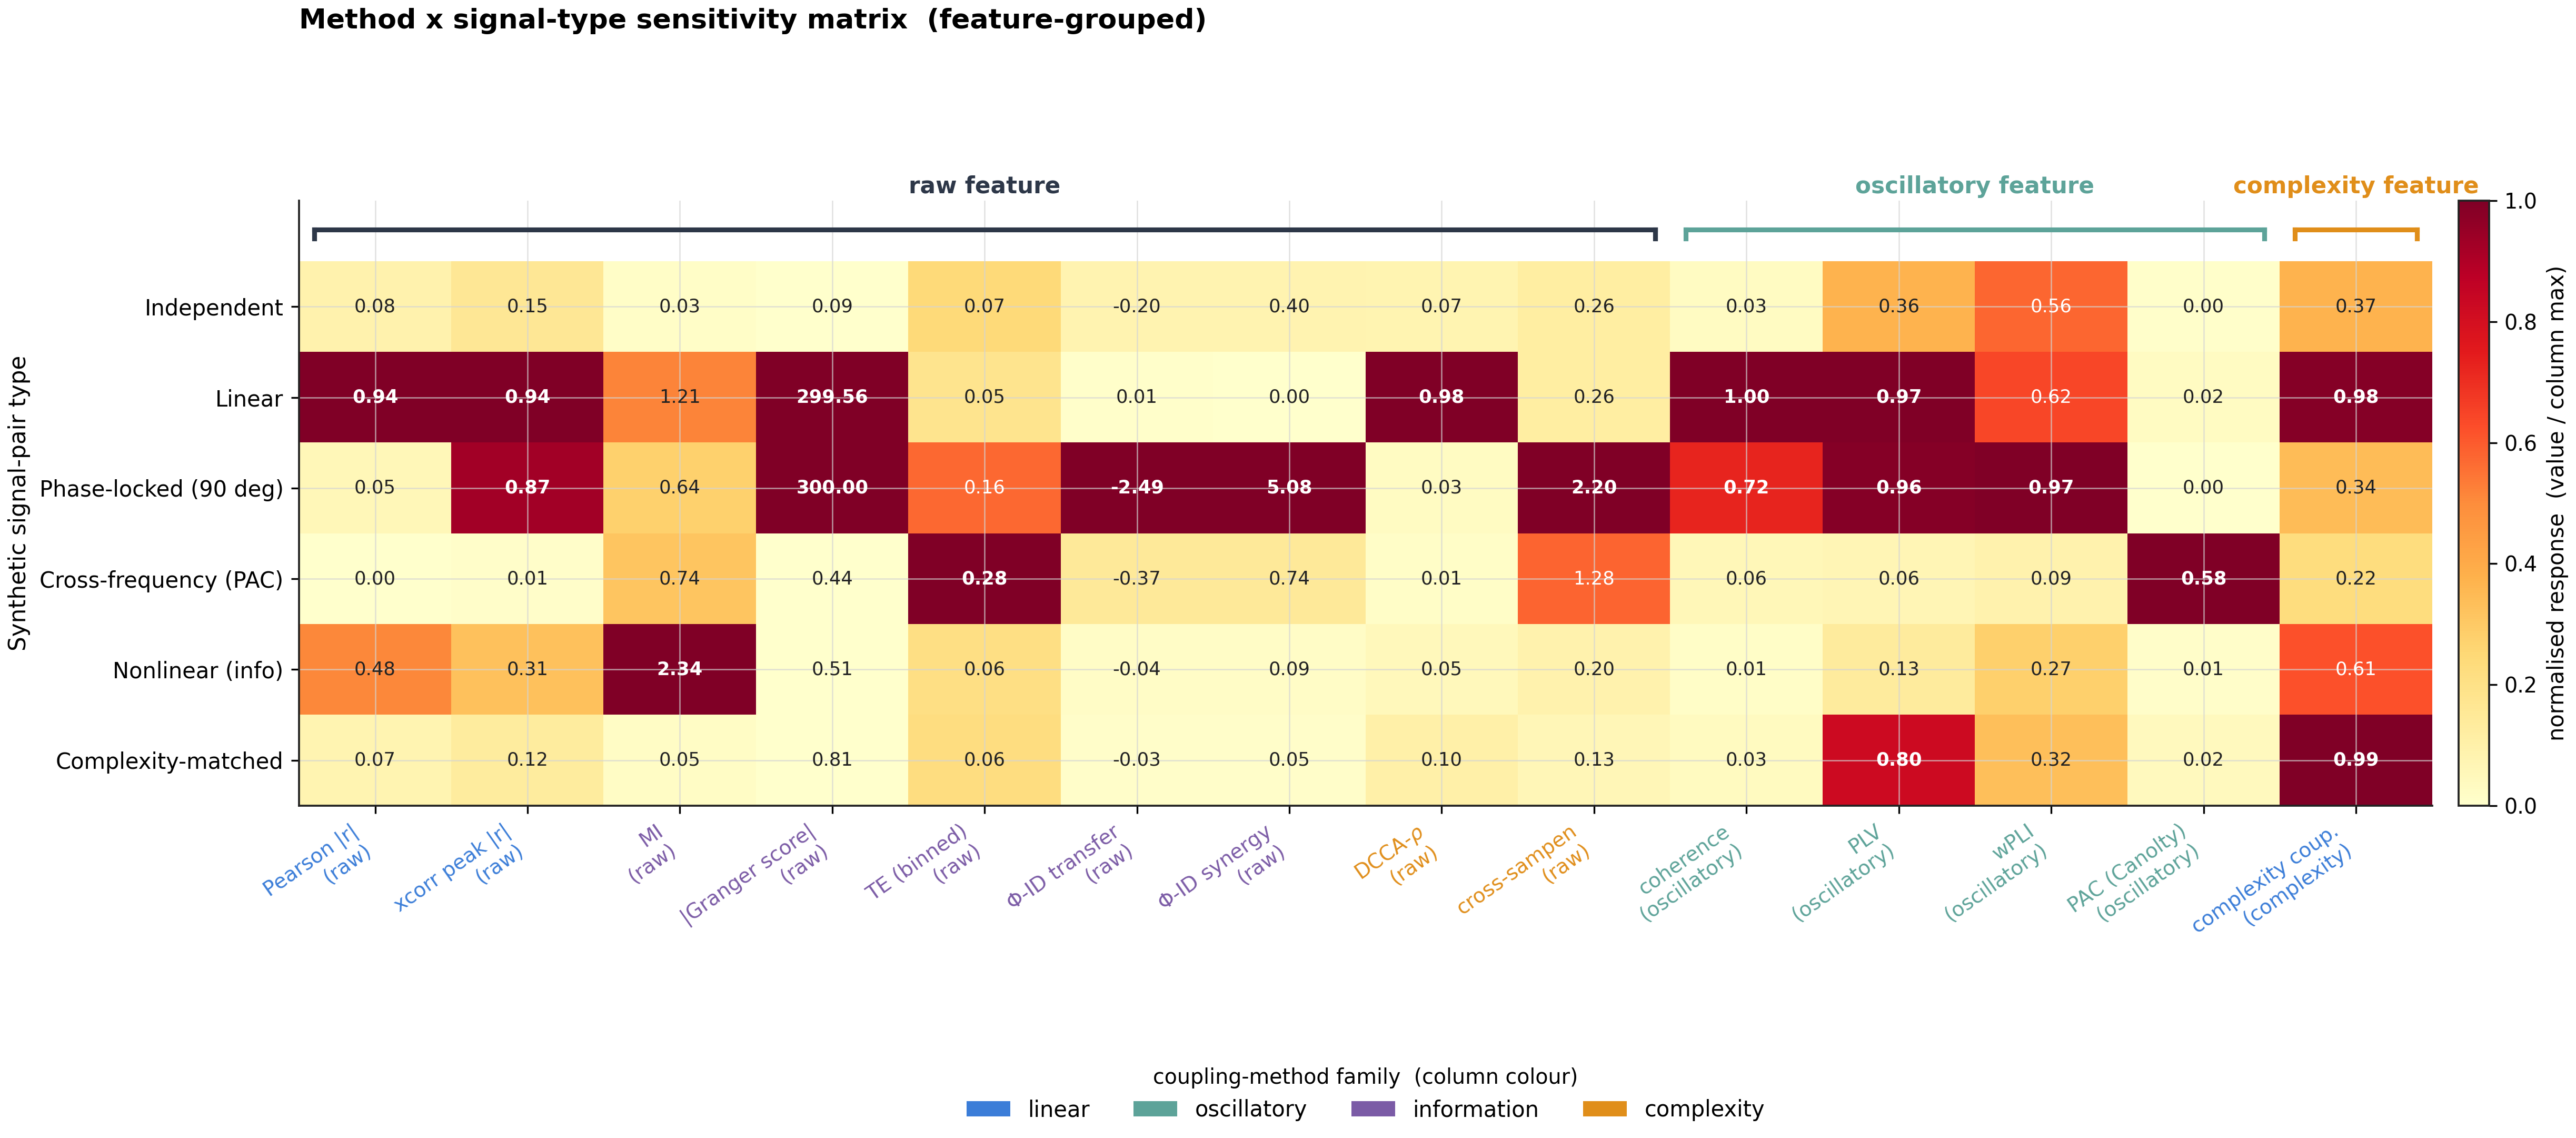
\includegraphics[width=\textwidth]{Methods2v2_sensitivity_matrix.png}
  \caption{\label{fig:matrix}\textbf{Method $\times$ signal-type
    sensitivity matrix, framework-grouped.} Rows: six synthetic
    signal-pair types with known coupling structure. Columns: nine
    canonical estimators \emph{grouped by feature axis} (raw,
    oscillatory, complexity --- bracket headers above the heatmap),
    with the method-name colour encoding the \emph{coupling-method
    axis} (linear blue / oscillatory teal / information purple). Each
    column thus reads as an explicit (feature, coupling) cell of the
    framework in Figure~\ref{fig:framework}. Cells are the raw metric
    value, column-normalised to each method's maximum across rows
    (annotation = actual raw value). Each method's peak is in the row
    of the coupling type it most directly tests.}
\end{figure}

\section{Worked example}

To anchor the toolbox in real measurements, Figure~\ref{fig:worked}
runs all four families on one cell of the pilot dataset: the audio
swell envelope (column \texttt{env\_swell\_0p2} of the merged
preprocessing table) versus cleaned respiration, for subject~02 in
the audio--visual MULTI condition (289\,s of recording).

\begin{figure}[H]
  \centering
  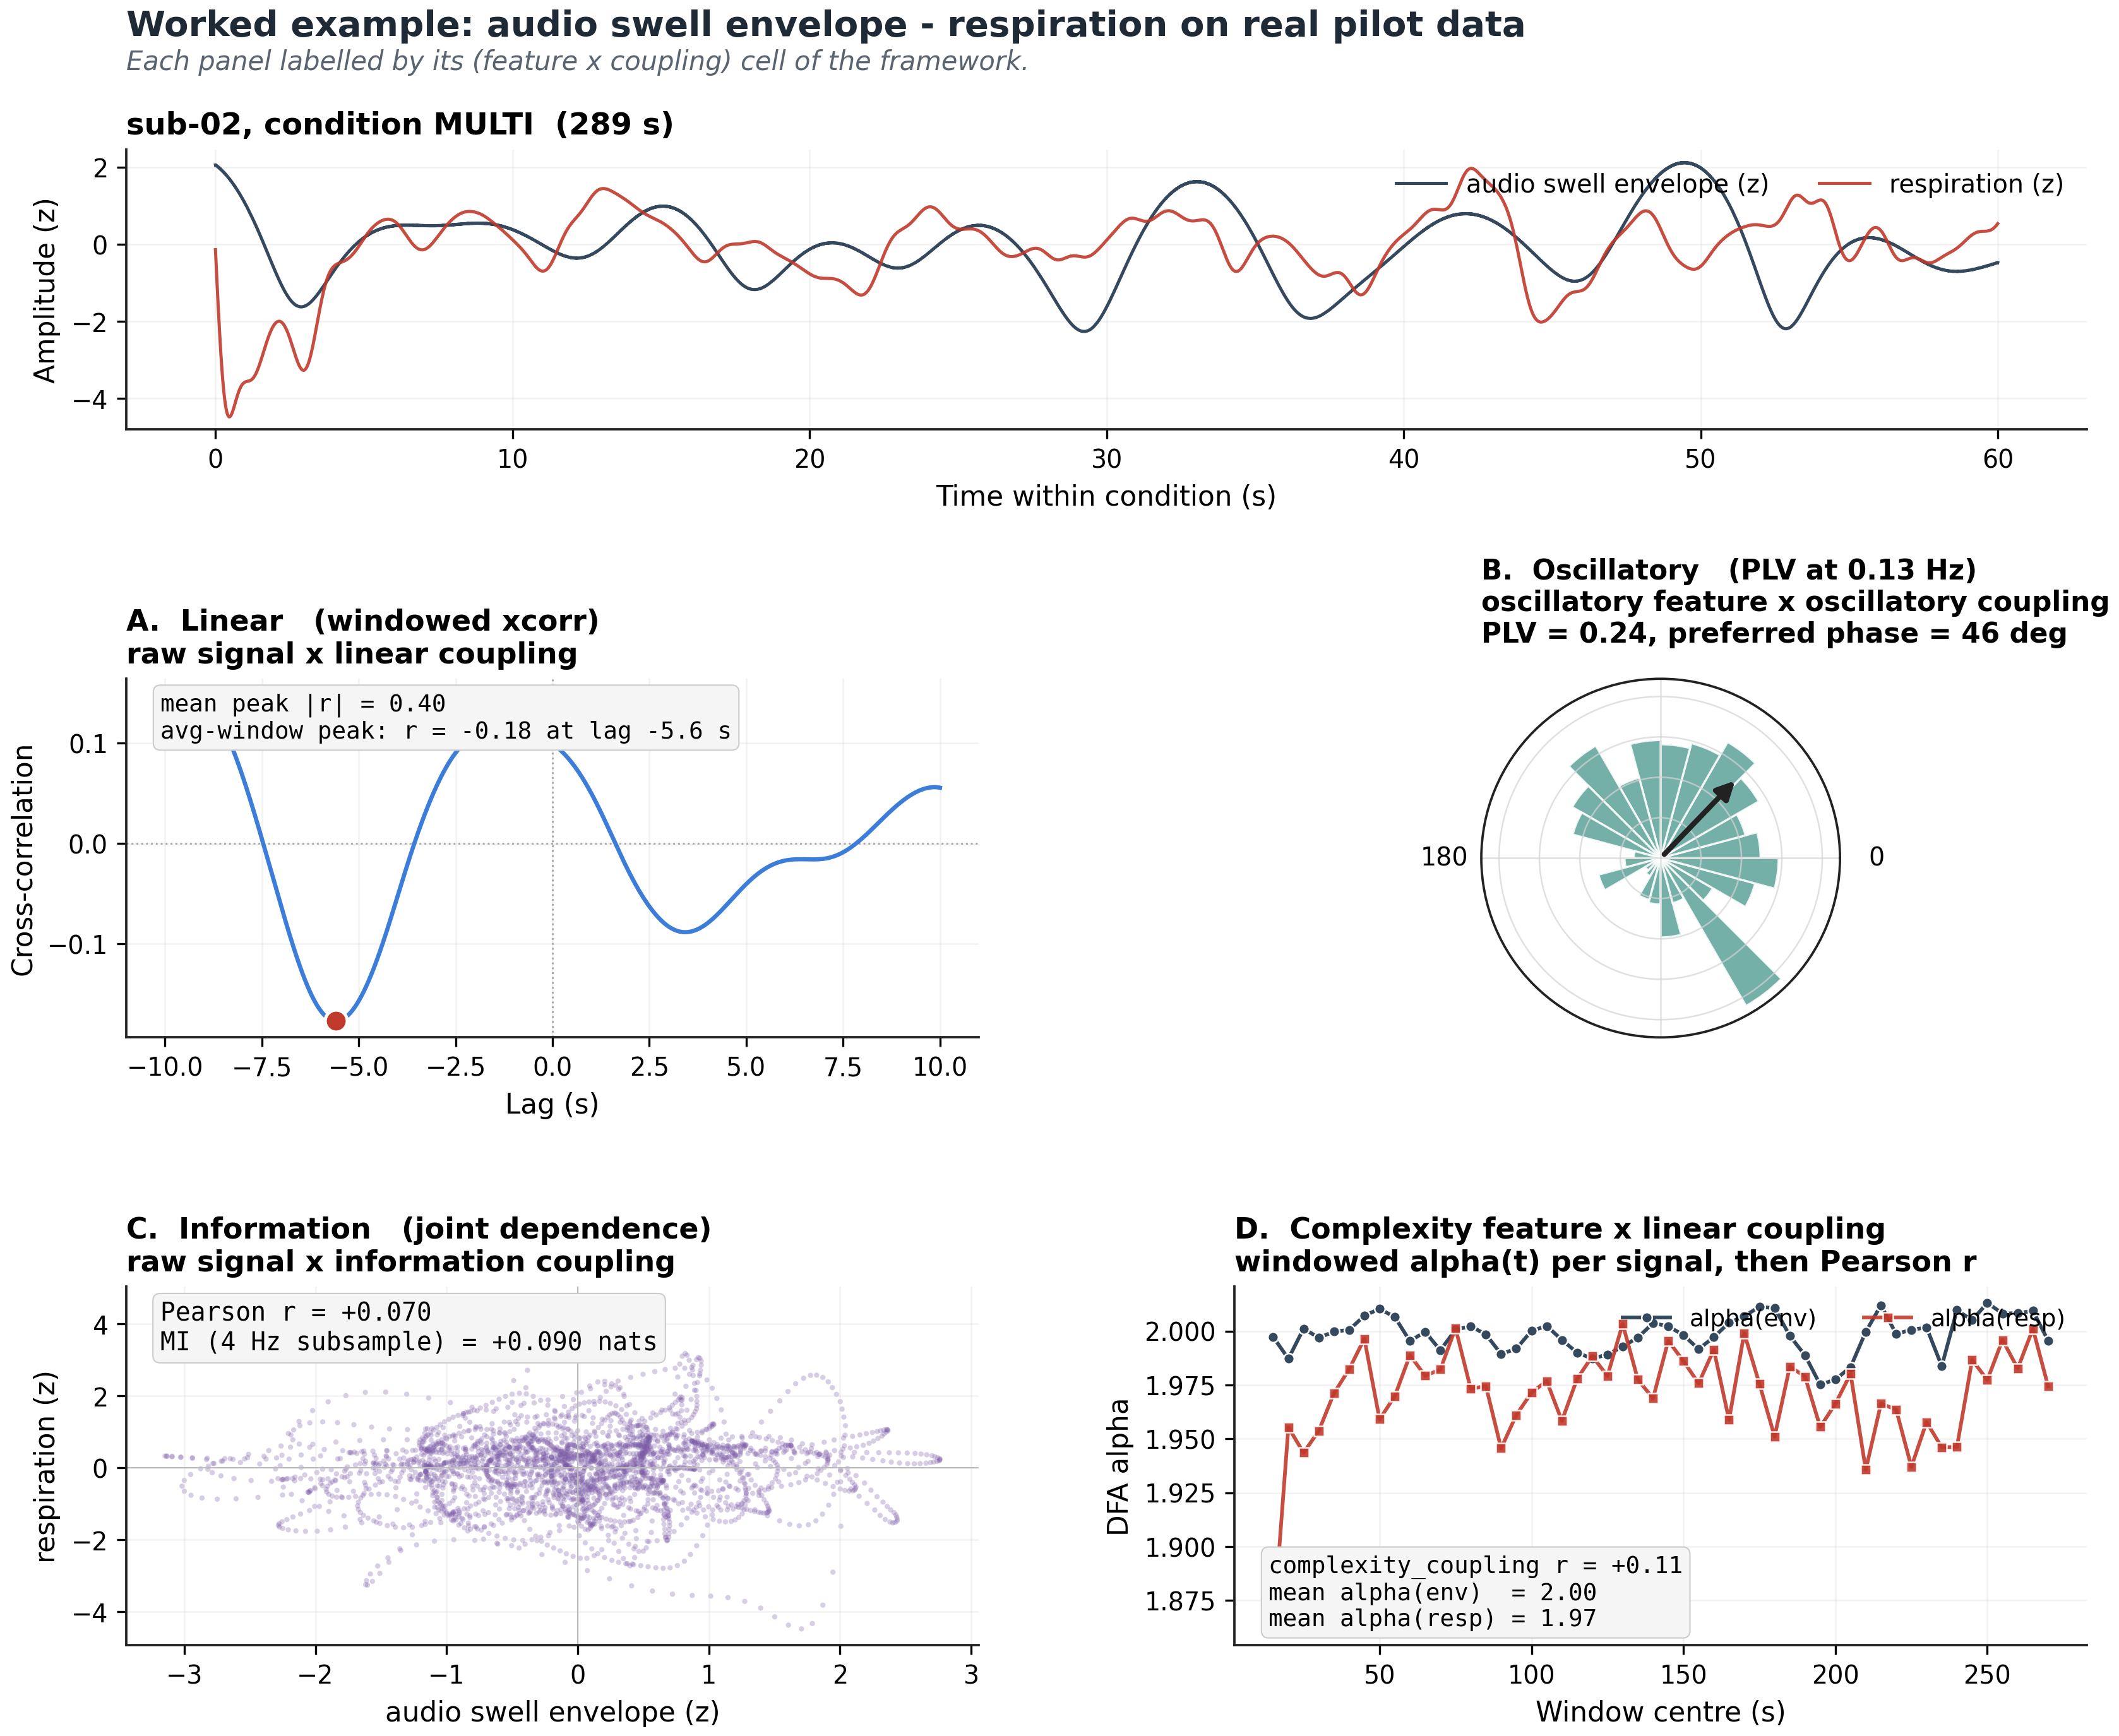
\includegraphics[width=\textwidth]{Methods6v2_worked_example.png}
  \caption{\label{fig:worked}\textbf{Worked example on real pilot
    data, framework-tagged.} sub-02, MULTI condition, audio swell
    envelope (slate) vs cleaned respiration (brick). Each panel is
    labelled with its (feature, coupling) cell of the framework. Top
    strip: 60\,s preview. \textbf{A. raw signal $\times$ linear} ---
    windowed xcorr; mean per-window peak $|r|$ is 0.40, with the
    average-window xcorr profile peaking at $\text{lag}=-5.6$\,s.
    \textbf{B. oscillatory feature $\times$ oscillatory} --- PLV at
    the auto-detected dominant frequency 0.13\,Hz is 0.24 with
    preferred phase $\approx 46^\circ$. \textbf{C. raw signal $\times$
    information} --- joint scatter; Pearson $r$ on a 4\,Hz subsample
    is near zero, MI is mildly positive. \textbf{D. complexity feature
    $\times$ linear} --- windowed DFA $\alpha$ traces hover near
    $\alpha\!=\!2$ for both signals (long-range correlated), and
    Pearson on the two $\alpha(t)$ traces is $r=0.11$ (weak coupling
    of complexity over time).}
\end{figure}

The reading is honest: this particular subject in this particular
condition shows modest, but non-zero, coupling on every method.
A group-level claim would require running the same pipeline across all
subjects and conditions, then a Friedman + Wilcoxon (small-$N$) or
LMM (windowed) analysis --- the templates for which live in
\texttt{scripts/figures/analysis\_nature\_vs\_rest.py}.

\section{Toolbox architecture}
\label{sec:toolbox-arch}

The current toolbox layout (see \texttt{src/HNA/README.md}) is a direct
realisation of the framework. The package is flat (importable as
\texttt{HNA.coupling.linear}, \texttt{HNA.features.fractal}, etc.) and
each subpackage's \texttt{\_\_init\_\_} re-exports the full public API.

A useful future refactor, suggested by the \(3 \times 3\) framework
matrix, is to consolidate today's scattered oscillatory-feature
extractors (\texttt{dsp.hilbert\_envelope},
\texttt{coupling.oscillatory.\_phase\_and\_amp},
\texttt{features.psd}) into a unified \texttt{features.oscillatory}
submodule, and to merge \texttt{features.fractal} +
\texttt{features.aperiodic} + \texttt{features.entropy} into a single
\texttt{features.complexity} subpackage that exposes \emph{both}
fractality and entropy estimators behind a uniform API. Once both
exist, every cell of Figure~\ref{fig:framework} can be expressed as a
single unified call:
\begin{lstlisting}
# (proposed future API)
result = couple(feature_x(x), feature_y(y), method=...)
\end{lstlisting}
The toolbox already supports this pattern through the existing
\texttt{coupling/} subpackage; the missing piece is the unified
feature-side dispatcher. This is the most natural Tier-3 refactor.

\section{Limitations and future extensions}
\label{sec:future}

\paragraph{Sample-size statistics.} The pilot study has $N\!=\!5$.
Group-level inference is therefore Friedman + paired-Wilcoxon (with
optional add-one cluster permutation on windowed traces) rather than a
hierarchical mixed-effects framework. The toolbox is set up to handle
both; the choice is sample-size driven, not method-driven.

\paragraph{A genuine complexity-coupling family.} The framework
(Figure~\ref{fig:framework}) deliberately has only three coupling
columns --- linear, oscillatory, information --- because every method
currently in the \texttt{coupling.complexity} subpackage is in fact a
linear comparison of complexity \emph{features}. A genuine
complexity-coupling family would contain estimators whose
\emph{coupling step} is itself non-linear and scale-aware. The natural
candidates are \textbf{Detrended Cross-Correlation Analysis
(DCCA)}~\cite{Podobnik2008}, which gives a joint scaling exponent for
two signals; \textbf{multiscale cross-entropy} and \textbf{cross sample
entropy} extensions of multiscale entropy~\cite{Costa2002} to bivariate
signals; and \textbf{multiscale cross-mutual-information}, which
applies kNN MI at successive coarse-graining levels. Adding any of
these promotes the framework to a \(3\!\times\!4\) grid in which the
``complexity'' column is genuinely populated rather than merely a
relabelling of linear coupling on a complexity feature. This is the
natural next addition to the toolbox.

\paragraph{Cross-modal complexity matching.} Even within the current
linear-on-complexity-feature framing, multiscale entropy matching
across modalities (e.g.\ EEG aperiodic exponent vs HRV $\alpha$) is
supported by \texttt{coupling.complexity.mse\_matching} and
\texttt{exponent\_matching} but has not been deployed across the full
pilot grid. This is high on the list for the second analysis pass.

\paragraph{Video.} The current toolbox is audio + EEG + ECG/HRV +
respiration. A \texttt{modalities.video} cleaner that exposes per-frame
luminance, optical flow, and frame-fractal-dimension as 1-D features
would slot directly into the framework: video features go in the same
\texttt{features.oscillatory} or \texttt{features.complexity} buckets,
and the existing coupling families couple them to physiology without
any further machinery.

\paragraph{Spectral Granger / partial Granger.} The toolbox ships
time-domain bivariate Granger only; spectral Granger and partial
(conditional) Granger are obvious extensions when the dataset grows
enough to support multivariate fits.

%--------------------------------------------------------------------
\bibliographystyle{unsrtnat}
\begin{thebibliography}{99}

\bibitem{Lachaux1999}
Lachaux JP, Rodriguez E, Martinerie J, Varela FJ.
Measuring phase synchrony in brain signals.
\emph{Hum Brain Mapp} 1999;8:194--208.

\bibitem{Vinck2011}
Vinck M, Oostenveld R, van Wingerden M, Battaglia F, Pennartz CM.
An improved index of phase-synchronization for electrophysiological data
in the presence of volume-conduction, noise and sample-size bias.
\emph{NeuroImage} 2011;55:1548--1565.

\bibitem{Tort2010}
Tort AB, Komorowski R, Eichenbaum H, Kopell N.
Measuring phase-amplitude coupling between neuronal oscillations of
different frequencies. \emph{J Neurophysiol} 2010;104:1195--1210.

\bibitem{Canolty2006}
Canolty RT, Edwards E, Dalal SS, Soltani M, Nagarajan SS, Kirsch HE,
Berger MS, Barbaro NM, Knight RT.
High gamma power is phase-locked to theta oscillations in human
neocortex. \emph{Science} 2006;313:1626--1628.

\bibitem{Kraskov2004}
Kraskov A, St\"ogbauer H, Grassberger P.
Estimating mutual information.
\emph{Phys Rev E} 2004;69:066138.

\bibitem{Schreiber2000}
Schreiber T.
Measuring information transfer.
\emph{Phys Rev Lett} 2000;85:461--464.

\bibitem{Peng}
Peng C-K, Buldyrev SV, Havlin S, Simons M, Stanley HE, Goldberger AL.
Mosaic organization of DNA nucleotides.
\emph{Phys Rev E} 1994;49:1685--1689.

\bibitem{Donoghue2020}
Donoghue T, Haller M, Peterson EJ, Varma P, Sebastian P, Gao R,
Noto T, Lara AH, Wallis JD, Knight RT, Shestyuk A, Voytek B.
Parameterizing neural power spectra into periodic and aperiodic
components. \emph{Nat Neurosci} 2020;23:1655--1665.

\bibitem{Costa2002}
Costa M, Goldberger AL, Peng C-K.
Multiscale entropy analysis of complex physiologic time series.
\emph{Phys Rev Lett} 2002;89:068102.

\bibitem{Podobnik2008}
Podobnik B, Stanley HE.
Detrended cross-correlation analysis: a new method for analyzing two
nonstationary time series.
\emph{Phys Rev Lett} 2008;100:084102.

\bibitem{Marmelat2012}
Marmelat V, Delign\`eres D.
Strong anticipation: complexity matching in interpersonal coordination.
\emph{Exp Brain Res} 2012;222:137--148.

\bibitem{MarisOostenveld2007}
Maris E, Oostenveld R.
Nonparametric statistical testing of EEG- and MEG-data.
\emph{J Neurosci Methods} 2007;164:177--190.

\bibitem{NK2}
Makowski D, Pham T, Lau ZJ, Brammer JC, Lespinasse F, Pham H,
Sch\"olzel C, Chen SHA.
NeuroKit2: A Python toolbox for neurophysiological signal processing.
\emph{Behav Res Methods} 2021;53:1689--1696.

\bibitem{Pichot}
Pichot V, Roche F, Celle S, Barth\'el\'emy J-C, Chouchou F.
HRVanalysis: a free software for analyzing cardiac autonomic activity.
\emph{Front Physiol} 2016;7:557.

\end{thebibliography}

\end{document}
